\section{积分换元}
\label{sec:integral-change-of-variables}

累次积分保留原来的坐标，只改变累计次序。换元则通过一个映射把积分搬到另一个空间：对输出空间上的函数求积分，能否改成对输入空间上的复合函数求积分？本节按映射所满足的条件逐层具体化。一般可测映射只携带测度，换元规则由第二章的推前测度给出；若映射是欧氏空间开集间的光滑可逆变换，输出测度可以用Jacobian行列式写成Lebesgue测度的加权形式；若映射只能分成若干可逆分支，就逐支换元再累计。这里的“换元”始终是两个空间之间的变量替换；第四章在同一空间上更换参考测度，那是另一种运算。

\subsection{可测映射下的换元}
\label{sec:integral-pushforward-change}

设$T:(X,\mathcal A)\to(Y,\mathcal B)$可测，$\mu$是$X$上的测度。第二章定义的推前测度（定义~\ref{def:measure-pushforward}）为$(T_\#\mu)(B)=\mu(T^{-1}(B))$：目标集合$B$得到的质量，是落进$B$的那些输入点的质量。现在要问，对$Y$上的函数$h$，积分$\int_Yh\,\mathrm d(T_\#\mu)$怎样回到输入空间计算。

先看示性函数$h=\mathbf 1_B$。左侧是$(T_\#\mu)(B)=\mu(T^{-1}(B))$；而$\mathbf 1_B(T(x))=1$当且仅当$x\in T^{-1}(B)$，所以$\mathbf 1_B\circ T=\mathbf 1_{T^{-1}(B)}$，右侧$\int_X\mathbf 1_B\circ T\,\mathrm d\mu$也等于$\mu(T^{-1}(B))$。沿积分的构造步骤推广，就得到一般结论。

\begin{theorem}[推前测度的积分换元]
\label{thm:integral-pushforward-change}
设$(X,\mathcal A,\mu)$是测度空间，$T:X\to Y$是$(\mathcal A,\mathcal B)$可测映射。
\begin{enumerate}
 \item 对每个可测$h:Y\to[0,\infty]$，
 \begin{equation}
  \int_Yh\,\mathrm d(T_\#\mu)=\int_Xh\circ T\,\mathrm d\mu,
  \label{eq:integral-pushforward-change}
 \end{equation}
 两侧可以同为$+\infty$。
 \item 对可测的实值或复值$h$，$h$关于$T_\#\mu$可积当且仅当$h\circ T$关于$\mu$可积，此时式~\eqref{eq:integral-pushforward-change}成立且两侧有限。
\end{enumerate}
\end{theorem}

\begin{proof}
$h\circ T$是可测映射的复合，因而可测（第~\ref{sec:measure-measurable-maps}节）。(1)示性函数的情形已在上面核对。对非负简单函数$s=\sum_ic_i\mathbf 1_{B_i}$，$s\circ T=\sum_ic_i\mathbf 1_{B_i}\circ T$，两侧由线性性相等。对一般非负可测$h$，取简单函数$s_n\uparrow h$，则$s_n\circ T\uparrow h\circ T$，两侧分别用单调收敛定理取极限。

(2)由$|h\circ T|=|h|\circ T$，把(1)用于$|h|$，两侧绝对积分相等，可积性等价。实值时$(h\circ T)^\pm=h^\pm\circ T$，对正部和负部分别用(1)后相减；复值时对实部和虚部分别处理。
\end{proof}

定理不要求$T$可逆、可微，甚至不要求两端有距离；它只用到可测性和推前测度的定义。式~\eqref{eq:integral-pushforward-change}可以从两个方向读：已知$\mu$时，用它计算输出空间上的积分；已知输出测度时，用它说明对复合函数$h\circ T$的累计只取决于$T$把质量送到了哪里。

\begin{example}[有限集合上的分组汇总]
\label{ex:integral-pushforward-finite}
取$X=\{1,2,3,4\}$，$\mu(\{k\})=k/10$；$Y=\{0,1\}$，$T(1)=T(3)=1$、$T(2)=T(4)=0$。输出点$0$的原像是$\{2,4\}$，所以$(T_\#\mu)(\{0\})=0.2+0.4=0.6$；同理$(T_\#\mu)(\{1\})=0.1+0.3=0.4$。取$h(0)=5$、$h(1)=2$，左侧是$5\times0.6+2\times0.4=3.8$；右侧逐个输入点计算$h(T(k))\mu(\{k\})$，得$2\times0.1+5\times0.2+2\times0.3+5\times0.4=3.8$。
\end{example}

图~\ref{fig:integral-pushforward-change}显示了两种算法的差别：右侧逐点累计，左侧先把映到同一输出点的输入质量合并，再乘以该点的函数值。多对一映射正是通过这种合并，把不同输入点的质量汇集到同一个输出点；整个计算没有用到任何“输出密度”，输出测度本身就是两个原子。

\begin{figure}[!htbp]
\centering
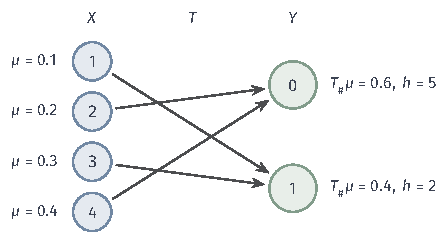
\includegraphics[width=75.812mm]{figures/02-abstract-mathematics/01-metric-and-measure/tikz/c3-pushforward-change/figure.pdf}
\caption{有限集合上的推前与换元。输入点$k=1,2,3,4$的质量为$k/10$，映射$T$把$2,4$送到$0$、把$1,3$送到$1$，输出质量分别为$0.6$与$0.4$。取$h(0)=5$、$h(1)=2$，按输出点汇总与按输入点逐个累计都得到$3.8$。}
\label{fig:integral-pushforward-change}
\end{figure}

由$(S\circ T)^{-1}(C)=T^{-1}(S^{-1}(C))$，推前满足$(S\circ T)_\#\mu=S_\#(T_\#\mu)$（第~\ref{sec:measure-pushforward}节），所以接连两次换元等于用复合映射一次换元，式~\eqref{eq:integral-pushforward-change}可以逐级使用。

\subsection{可逆光滑变换下的换元}
\label{sec:integral-jacobian-change}

当$X,Y$都是$\mathbb R^d$中的开集、$\mu=\lambda_d$时，定理~\ref{thm:integral-pushforward-change}把$\int h\circ T\,\mathrm d\lambda_d$转化为对推前测度$T_\#\lambda_d$的积分，但还没有说$T_\#\lambda_d$长什么样。若$T$光滑可逆，局部看来它近似一个线性变换，体积按一个确定的比例改变，这个比例就是Jacobian行列式的绝对值。

\paragraph{Jacobian换元公式}
设$U,V\subseteq\mathbb R^d$为开集。若$T:U\to V$是双射，$T$与$T^{-1}$都连续可微，则称$T$为\term{微分同胚}（diffeomorphism），更准确地说是$C^1$微分同胚。对$T^{-1}\circ T=\mathrm{id}$求导得$DT^{-1}(T(\bm x))DT(\bm x)=\bm I$，所以$\det DT(\bm x)\ne0$处处成立；$\det DT$称为$T$的\term{Jacobian行列式}（Jacobian determinant）。卷一在多元积分一章对紧Jordan区域上的连续函数证明了经典换元公式：若$E\subseteq U$是紧Jordan区域且$T(E)$也是Jordan区域，$f$在$T(E)$上连续，则$\int_{T(E)}f(\bm y)\,\mathrm d\bm y=\int_Ef(T(\bm x))|\det DT(\bm x)|\,\mathrm d\bm x$。现在把它推广到一般可测函数。

\begin{theorem}[可逆光滑变换下的换元]
\label{thm:integral-jacobian-change}
设$U,V\subseteq\mathbb R^d$为开集，$T:U\to V$是$C^1$微分同胚。对每个Lebesgue可测$h:V\to[0,\infty]$，
\begin{equation}
 \int_Vh(\bm y)\,\mathrm d\bm y=\int_Uh(T(\bm x))\,|\det DT(\bm x)|\,\mathrm d\bm x,
 \label{eq:integral-jacobian-change}
\end{equation}
两侧可以同为$+\infty$。若$h$是实值或复值Lebesgue可测函数，则$h$在$V$上可积当且仅当$(h\circ T)|\det DT|$在$U$上可积，此时式~\eqref{eq:integral-jacobian-change}成立且两侧有限。
\end{theorem}

\begin{proof}
论证的任务是把经典公式中的“连续函数、Jordan区域”换成“可测函数、可测集合”。分四步进行。

第一步，构造比较对象。对Borel集$B\subseteq V$，令
\[
 \rho(B)=\int_U\mathbf 1_B(T(\bm x))\,|\det DT(\bm x)|\,\mathrm d\bm x.
\]
$T$连续，$\mathbf 1_B\circ T$是Borel函数；$|\det DT|$连续，因而可测。若$B_n$两两不交，$\mathbf 1_{\bigcup_nB_n}\circ T=\sum_n\mathbf 1_{B_n}\circ T$，非负级数可以逐项积分，所以$\rho$是$V$的Borel集上的测度。式~\eqref{eq:integral-jacobian-change}对示性函数说的正是$\rho=\lambda_d$。

第二步，在闭盒上比较。设$Q\subseteq V$是闭盒（允许退化）。$E=T^{-1}(Q)$是紧集，因为$T^{-1}$连续；$T^{-1}$是同胚，所以$E$的边界是$T^{-1}(\partial Q)$。$\partial Q$的Jordan容量为零，$T^{-1}$在$Q$的一个紧邻域上Lipschitz，把容量为零的集合映成容量为零的集合，故$E$是紧Jordan区域。对$f\equiv1$应用经典公式，得$\lambda_d(Q)=\int_E|\det DT|\,\mathrm d\bm x=\rho(Q)$；这里Jordan区域上连续函数的Riemann积分等于Lebesgue积分（第~\ref{sec:integral-classical}节）。

第三步，推广到Borel集与非负Borel函数。含于$V$的闭盒对有限交封闭（交集是闭盒或空集），$V$的每个开子集都是可数个含于其中的有理端点闭盒之并，所以它们生成$V$上的Borel $\sigma$代数，并且可数个这样的闭盒覆盖$V$，各自测度有限。由$\pi$--$\lambda$唯一性（定理~\ref{thm:measure-pi-lambda}），$\rho=\lambda_d$在$V$的Borel集上成立。由线性性，式~\eqref{eq:integral-jacobian-change}对非负Borel简单函数成立；取递增逼近并在两侧用单调收敛定理，它对非负Borel函数成立。

第四步，推广到Lebesgue可测函数。Lebesgue可测结构是Borel测度的完备化，因此非负Lebesgue可测$h$与某个非负Borel函数$\tilde h$只在一个Borel零测集$N\subseteq V$内不同。对$\mathbf 1_N$用第三步，$\int_U\mathbf 1_N(T(\bm x))|\det DT(\bm x)|\,\mathrm d\bm x=\lambda_d(N)=0$；被积函数非负、积分为零，所以它几乎处处为零，又因$|\det DT|>0$，得$\lambda_d(T^{-1}(N))=0$。于是$h\circ T$与$\tilde h\circ T$只在零测集上不同，前者Lebesgue可测，并且两侧积分分别与$\tilde h$的相应积分相同。实值或复值情形先对$|h|$使用非负结论确认可积性等价，再对正负部或实部、虚部分别使用。
\end{proof}

定理中的条件分别承担不同的任务：$C^1$保证局部体积比例由$|\det DT|$连续地描述，双射保证每块输出区域只被一个输入区域覆盖一次。若在正测度的区域上发生重叠，单一的换元公式会少算或多算质量，这是下一小节的问题。

\paragraph{线性变换与体积比例}
最简单的情形是仿射变换$T(\bm x)=\bm A\bm x+\bm b$，其中$\bm A$为可逆$d\times d$矩阵。此时$DT\equiv\bm A$，Jacobian因子是常数$|\det\bm A|$。对可测集$E\subseteq\mathbb R^d$，在式~\eqref{eq:integral-jacobian-change}中取$h=\mathbf 1_{T(E)}$，左侧是$\lambda_d(T(E))$，右侧是$\int_E|\det\bm A|\,\mathrm d\bm x$，于是
\[
 \lambda_d(\bm AE+\bm b)=|\det\bm A|\,\lambda_d(E).
\]
线性变换的行列式绝对值是固定的体积比例，平移的比例为$1$。图~\ref{fig:integral-jacobian-cell}中$\bm A=\begin{bmatrix}1.5&0.5\\0.5&1\end{bmatrix}$把单位正方形变成以两列为边的平行四边形，面积$|1.5\times1-0.5\times0.5|=1.25$；取绝对值是因为反射等改变定向的变换行列式为负，而面积非负。对一般的$C^1$微分同胚，$\bm x$附近的小块被近似地按$DT(\bm x)$线性变换，$|\det DT(\bm x)|$就是这一点处的局部体积比例。

\begin{figure}[!htbp]
\centering
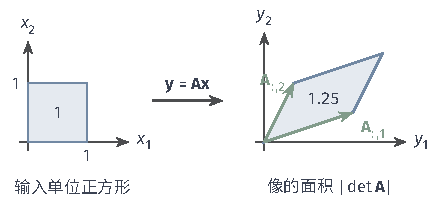
\includegraphics[width=74.701mm]{figures/02-abstract-mathematics/01-metric-and-measure/tikz/c3-jacobian-cell/figure.pdf}
\caption{可逆线性变换的体积比例。$\bm A=\begin{bmatrix}1.5&0.5\\0.5&1\end{bmatrix}$把面积为$1$的单位正方形映成以列向量$\bm A_{:,1}=(1.5,0.5)^\top$、$\bm A_{:,2}=(0.5,1)^\top$为边的平行四边形，面积为$|\det\bm A|=1.25$。}
\label{fig:integral-jacobian-cell}
\end{figure}

\begin{example}[极坐标与Gauss积分]
\label{ex:integral-polar-gauss}
令$U=(0,\infty)\times(0,2\pi)$，$T(r,\theta)=(r\cos\theta,r\sin\theta)$，$V=\mathbb R^2\setminus\{(x,0):x\ge0\}$。$T:U\to V$是$C^1$微分同胚，$\det DT(r,\theta)=r$。被去掉的射线是$\lambda_2$零测集（它包含在矩形$[0,\infty)\times\{0\}$中，测度为$\infty\cdot0=0$），不影响积分。取$h(x,y)=e^{-(x^2+y^2)}$，
\[
 \int_{\mathbb R^2}e^{-(x^2+y^2)}\,\mathrm d\lambda_2=\int_0^{2\pi}\!\!\int_0^\infty e^{-r^2}r\,\mathrm dr\,\mathrm d\theta=2\pi\cdot\frac12=\pi,
\]
右侧的累次积分由Tonelli定理得到。另一方面，左侧的被积函数是$e^{-x^2}e^{-y^2}$，Tonelli定理给出它等于$\bigl(\int_{\mathbb R}e^{-x^2}\,\mathrm dx\bigr)^2$，于是$\int_{\mathbb R}e^{-x^2}\,\mathrm dx=\sqrt\pi$。
\end{example}

Jacobian公式只是在通用换元关系~\eqref{eq:integral-pushforward-change}的基础上，对可逆光滑变换进一步识别了体积如何变化。一般可测映射不满足它的条件：$T$不可逆时输出可能重叠，$T$把$\mathbb R^d$映到低维集合时输出集合的$d$维体积为零。后一种情形需要曲线、曲面上的面积测度或余面积公式，留给相应的几何内容。

\subsection{分支可逆变换下的换元}
\label{sec:integral-branch-change}

许多常用变换不是整体可逆的，但可以分成几段，每段可逆。例如$T(x)=x^2$在$(-1,1)$上把$x$与$-x$送到同一点，在$(0,1)$和$(-1,0)$上却分别是微分同胚。对这类映射，把输入区域分开，逐支应用上一小节的定理，再把结果加起来。

\begin{theorem}[分支可逆变换下的换元]
\label{thm:integral-branch-change}
设$U\subseteq\mathbb R^d$为开集，$N\subseteq U$是Lebesgue零测集，$U\setminus N$是有限或可数个两两不交开集$U_k$之并；设$T:U\to\mathbb R^d$在每个$U_k$上的限制$T_k:U_k\to V_k=T(U_k)$都是开集之间的$C^1$微分同胚。则对每个Lebesgue可测$f:U\to[0,\infty]$，
\begin{equation}
 \int_Uf(\bm x)\,\mathrm d\bm x=\sum_k\int_{V_k}f\bigl(T_k^{-1}(\bm y)\bigr)\,\bigl|\det DT_k^{-1}(\bm y)\bigr|\,\mathrm d\bm y.
 \label{eq:integral-branch-change}
\end{equation}
若$f$是实值或复值可积函数，上式右侧的级数绝对收敛，等式仍成立。
\end{theorem}

\begin{proof}
零测集不影响积分，$\int_Uf=\int_{U\setminus N}f$。$U\setminus N$是两两不交的$U_k$之并，$f\mathbf 1_{U\setminus N}=\sum_kf\mathbf 1_{U_k}$，非负级数可以逐项积分，故$\int_Uf=\sum_k\int_{U_k}f$；可数个分支的累计正是由单调收敛保证的。对第$k$项，把定理~\ref{thm:integral-jacobian-change}用于微分同胚$T_k^{-1}:V_k\to U_k$和$U_k$上的函数$f$，得到
\[
 \int_{U_k}f(\bm x)\,\mathrm d\bm x=\int_{V_k}f\bigl(T_k^{-1}(\bm y)\bigr)\,\bigl|\det DT_k^{-1}(\bm y)\bigr|\,\mathrm d\bm y.
\]
相加即得式~\eqref{eq:integral-branch-change}。可积情形先对$|f|$使用非负结论，得到右侧绝对收敛，再对正负部或实部、虚部分别处理。
\end{proof}

式~\eqref{eq:integral-branch-change}右侧是对分支求和，不是在输出空间上选一个逆。各分支的像$V_k$可以重叠：若某点$\bm y$同时属于$V_1$和$V_2$，它有两个原像，两项都要计入；只选择一个逆分支，就会漏掉另一个原像那里的质量。把$f=h\circ T$代入就能看清这一点：
\[
 \int_Uh(T(\bm x))\,\mathrm d\bm x=\int h(\bm y)\sum_k\mathbf 1_{V_k}(\bm y)\,\bigl|\det DT_k^{-1}(\bm y)\bigr|\,\mathrm d\bm y,
\]
输出点$\bm y$的权重是它所有原像分支的体积比例之和。另一个条件是被扔掉的$N$必须零测。若某一部分输入区域没有纳入任何分支且测度为正，例如$T$在一段区间上取常值，那部分的积分要另外计算，不能直接删去；单个微分同胚的情形既没有重叠，也没有剩余部分，所以不需要这两项检查。

\begin{example}[平方映射的两个分支]
\label{ex:integral-square-branches}
取$U=(-1,1)$，$T(x)=x^2$，$N=\{0\}$，$U_1=(0,1)$、$U_2=(-1,0)$，两支的像都是$V_1=V_2=(0,1)$，如图~\ref{fig:integral-branch-inverse}。逆分支为$T_1^{-1}(y)=\sqrt y$与$T_2^{-1}(y)=-\sqrt y$，导数分别是$1/(2\sqrt y)$与$-1/(2\sqrt y)$，绝对值都是$1/(2\sqrt y)$。式~\eqref{eq:integral-branch-change}给出
\[
 \int_{-1}^1f(x)\,\mathrm dx=\int_0^1\frac{f(\sqrt y)+f(-\sqrt y)}{2\sqrt y}\,\mathrm dy.
\]
取$f\equiv1$，左侧为$2$，右侧为$\int_0^1y^{-1/2}\,\mathrm dy=\bigl[2\sqrt y\bigr]_0^1=2$。若只用一个逆分支，右侧只剩$1$，恰好漏掉$(-1,0)$上的质量。原点处导数为零，$T$在那里不是局部微分同胚，但$\{0\}$零测，把它放进$N$不影响结果。再取$f(x)=x^2$检验：左侧为$2/3$，右侧为$\int_0^1\frac{2y}{2\sqrt y}\,\mathrm dy=\int_0^1y^{1/2}\,\mathrm dy=2/3$。第四章还会用同一个变换计算输出测度的密度。
\end{example}

\begin{figure}[!htbp]
\centering
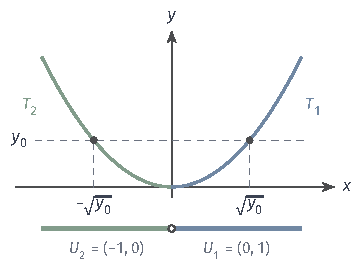
\includegraphics[width=61.33mm]{figures/02-abstract-mathematics/01-metric-and-measure/tikz/c3-branch-inverse/figure.pdf}
\caption{平方映射$T(x)=x^2$在$(-1,1)$上的两个可逆分支。蓝色分支$T_1$定义在$U_1=(0,1)$上，绿色分支$T_2$定义在$U_2=(-1,0)$上，空心点$x=0$是被去掉的零测集。水平线$y=y_0$与两个分支分别交于$\sqrt{y_0}$与$-\sqrt{y_0}$，所以每个输出值都要累计两个原像的贡献。}
\label{fig:integral-branch-inverse}
\end{figure}
